\section{PicoBlaze}
\begin{minipage}{9cm}
	\vspace{-4ex}
	Der PicoBlaze ist ein 8-Bit-RISC-Mikrocontroller-Kern. Er ist limitiert auf \textbf{1K Instruktionen}, besitzt von Grund auf nur das Carry- und Zero-Flag und verzichtet auf den Software-Stack.

Beim PicoBlaze kann mit der Clock-Frequenz bis hinunter zu 0Hz gefahren werden und alle Instruktionen werden immer in zwei Taktzyklen ausgef"uhrt.

Der PicoBlaze ist in einem FPGA eingebettet und bietet somit die optimale Balance zwischen den beiden.
\end{minipage}
%
\begin{minipage}{0.5cm}
	\ \
\end{minipage}
%
\begin{minipage}{8cm}
	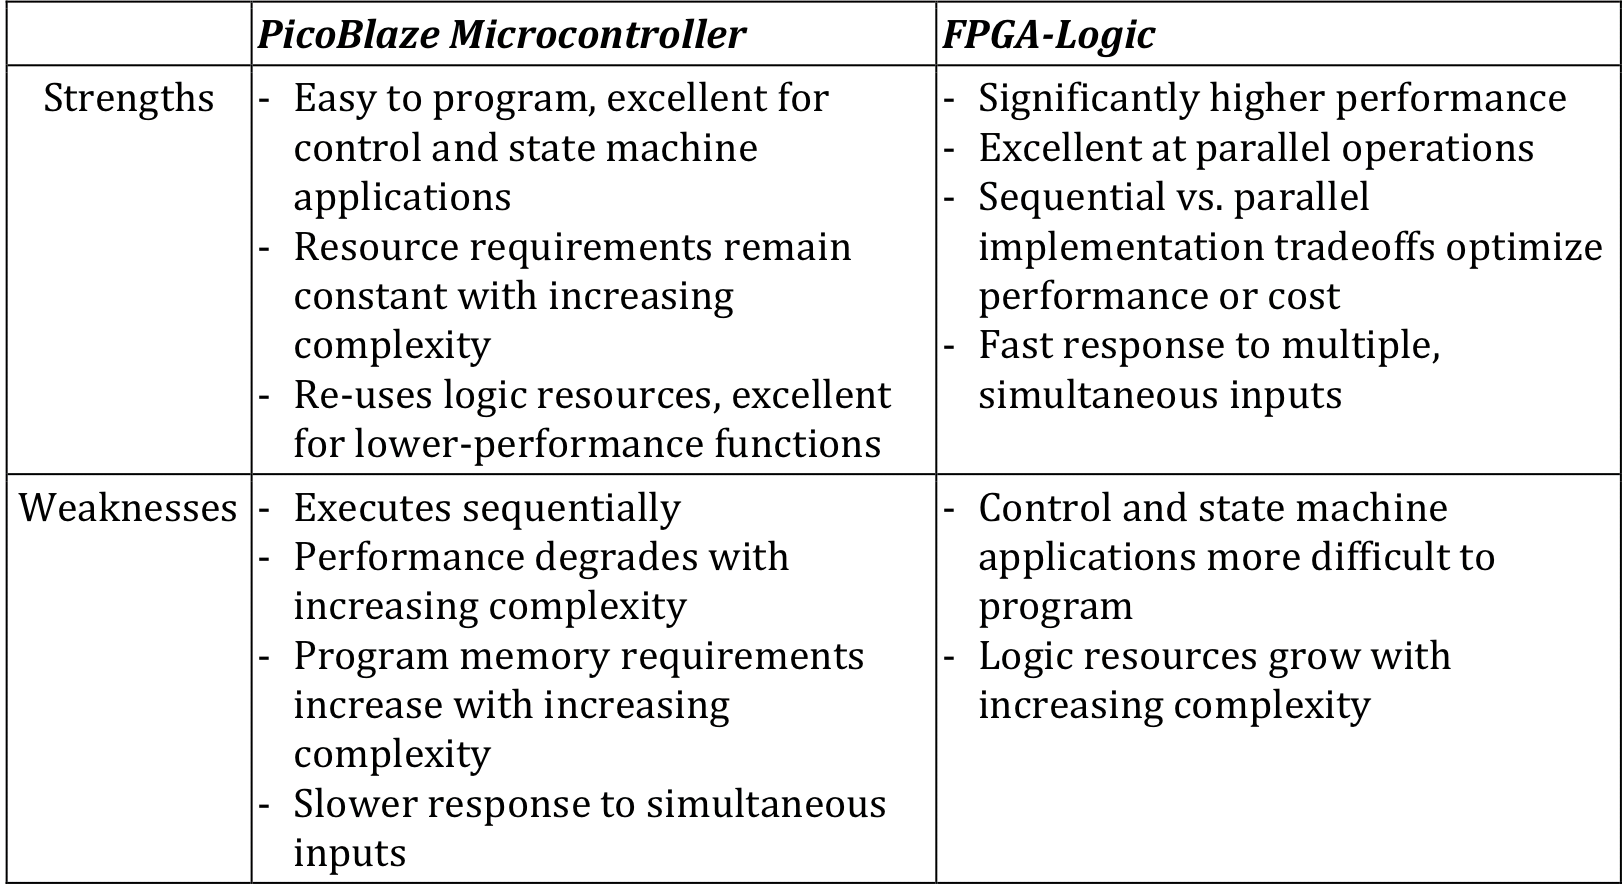
\includegraphics[width=8cm]{pics/PicoBlaze-Pro-Cons}
\end{minipage}

\subsection{Aufbau} 
\begin{minipage}{9cm}
	\vspace{-12ex}
	Der PicoBlaze verf"ugt "uber 16 \textbf{General-Purpose Register}, welche alle 8-Bit breit sind.
 	Die Verarbeitungsgr"osse der ALU betr"agt 8Bit, dabei werden alle operationen mit einem General-Purpose Regsiter (sX) als ersten Operanden durchgef"uhrt, das Resultat der Operation wird im selben Register (sX) abgelegt.
\end{minipage}
%
\begin{minipage}{0.5cm}
	\ \
\end{minipage}
%
\begin{minipage}{9cm}
	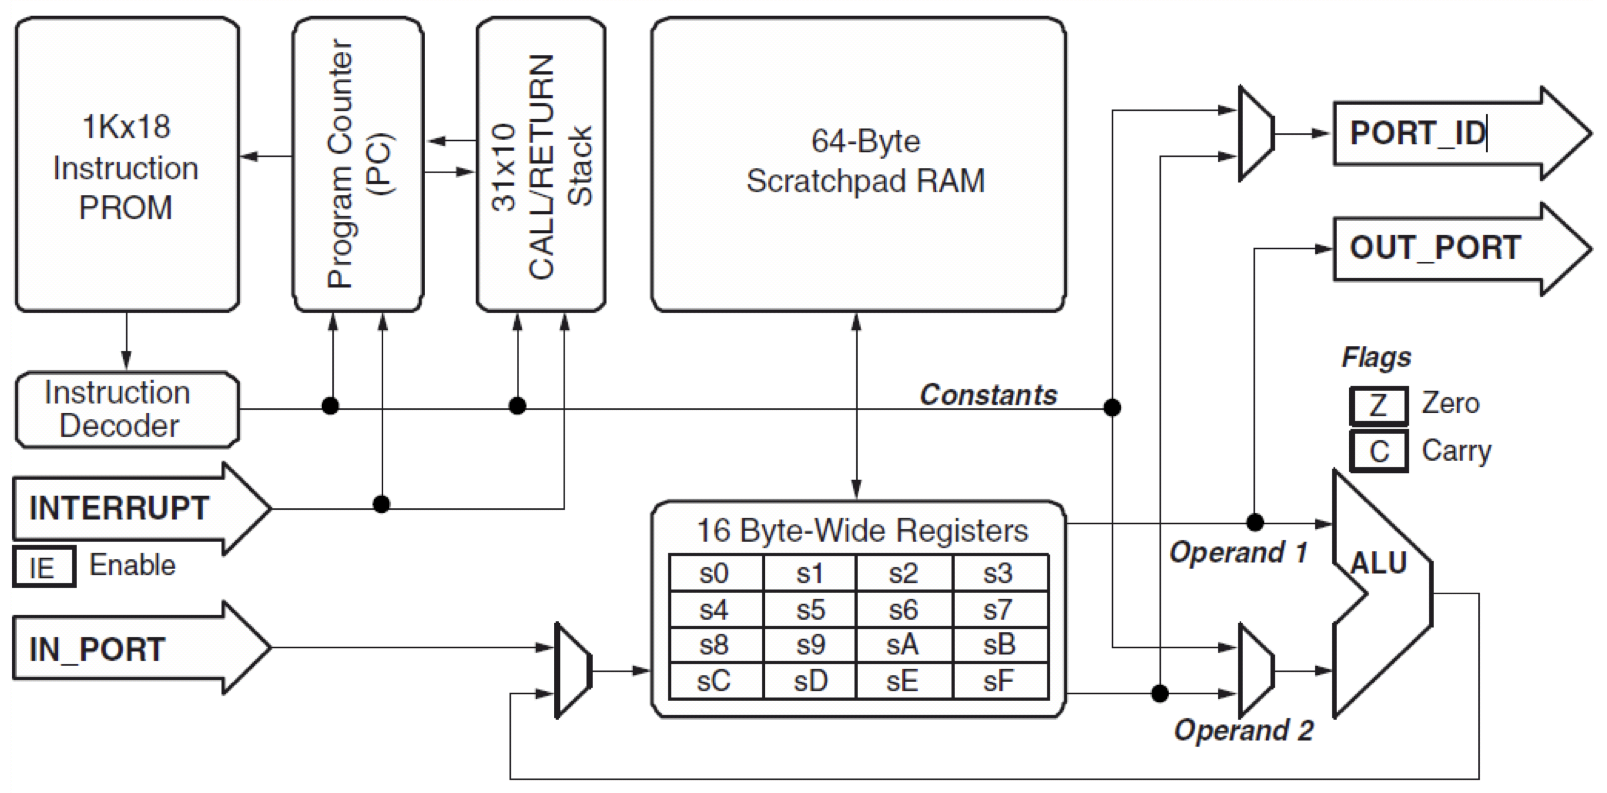
\includegraphics[width=9cm]{pics/PicoBlaze-Aufbau}
\end{minipage}
  
\subsection{Instruktionssatz}
\begin{minipage}{9cm}
	Alle Instruktionen des PicoBlaze Mikrocontrollers sind in einem einheitlich breiten Bitmuster, n"amlich 18 Bit breit. Dabei sind die Instruktionen als 0-, 1- oder 2-Adress-Befehle implementiert, wobei f"ur den Operand 1 bzw. Operand 2 je nach Instruktion unterschiedliche Angaben ben"otigen. Die Spezifikation eines Operanden kann ein direkter Zahlenwert sein oder sich auf die Bezeichnung ind den verschiedenen Adressbereichen beziehen.\\

	Der PicoBlaze hat nur wenige Adressbereiche, wie "ublich f"ur RISC-Prozessorkerne. Auf diese Adressbereiche kann nur mit klar festgelegten Instruktionsklassen und zugeh"origen Adressierungsarten zugegriffen werden.
\end{minipage}
%
\begin{minipage}{0.5cm}
	\ \
\end{minipage}
%
\begin{minipage}{9cm}
	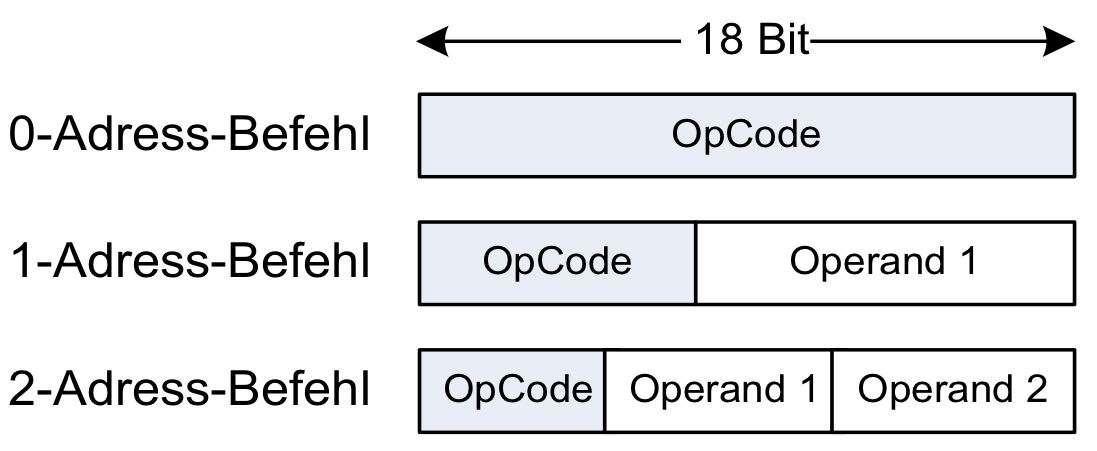
\includegraphics[width=5cm]{pics/PicoBlaze-OpGroesse}\\
	
	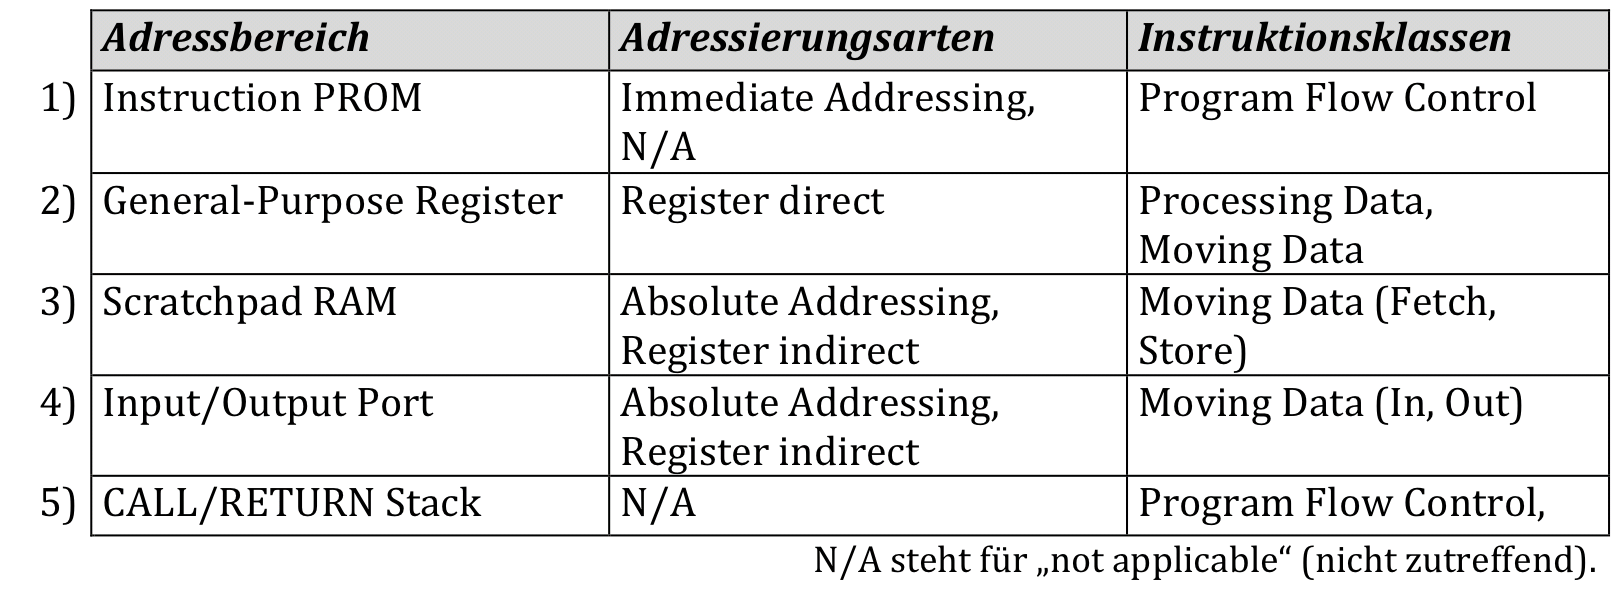
\includegraphics[width=8cm]{pics/PicoBlaze-Adressierung}
\end{minipage}

\subsection{Instruktionscodierung}
\begin{minipage}{9cm}
	Die Informationen zu den Operanden ist immer in den gleichen Bit-Bereichen lokalisiert. Bei der Disassemblierung von Instruction Codes gehen Kommentare und Labels verloren. Die Instruction Codes werden immer als Hexadezimale dargestellt. Mit den obersten 6-Bit (17-12) des Instruction Codes kann mit dem PicoBlaze Instruction Set (Quick-Reference) der Befehl lokalisiert werden.
\end{minipage}
%
\begin{minipage}{0.5cm}
	\ \
\end{minipage}
%
\begin{minipage}{9cm}
		\begin{tabular}{|l|l|l}
			\cline{1-2}
			\rowcolor[HTML]{C0C0C0} 
			\textbf{Operanden-Information} & \textbf{Bit}        & \cellcolor[HTML]{FFFFFF}{\color[HTML]{FFFFFF} \textbf{}} \\ \cline{1-2}
			Register sX                    & 11-8                        & \cellcolor[HTML]{F8FF00}x                                \\ \cline{1-2}
			Register sY                    & 7-4                         & \cellcolor[HTML]{34FF34}y                                \\ \cline{1-2}
			Absolute instruction address   & 9-0                         & \cellcolor[HTML]{34CDF9}a                                \\ \cline{1-2}
			Immediate Constant             & 7-0 						& \cellcolor[HTML]{F8A102}k                                \\ \cline{1-2}
			Port address                   & 7-0                         & \cellcolor[HTML]{FF00A9}p                                \\ \cline{1-2}
			Scratchpad RAM address         & 5-0                         & \cellcolor[HTML]{9B9B9B}s                                \\ \cline{1-2}
		\end{tabular}
\end{minipage}

\textbf{Beispiele:}
\begin{table}[h!]
\begin{tabular}{|lll|lll|llllll|}
\hline
\multicolumn{3}{|l|}{\cellcolor[HTML]{C0C0C0}\textbf{Assembler-Befehl}}                  & \multicolumn{3}{l|}{\cellcolor[HTML]{C0C0C0}\textbf{Syntax-Grundform}} & \multicolumn{6}{l|}{\cellcolor[HTML]{C0C0C0}\textbf{Instruction Code}}                                                                                                                                                         \\ \hline
IN    & \cellcolor[HTML]{F8FF00}s3  & \cellcolor[HTML]{34FF34}s9                         & IN      & \cellcolor[HTML]{F8FF00}sX,   & \cellcolor[HTML]{34FF34}sY   & 000101 & \cellcolor[HTML]{F8FF00}00                        & \cellcolor[HTML]{F8FF00}11                        & \cellcolor[HTML]{34FF34}10 & \cellcolor[HTML]{34FF34}01 & 0000                                                \\ \hline
SUB   & \cellcolor[HTML]{F8FF00}s3, & \cellcolor[HTML]{F8A102}{\color[HTML]{000000} 100} & SUB     & \cellcolor[HTML]{F8FF00}sX,   & \cellcolor[HTML]{F8A102}kk   & 011100 & \cellcolor[HTML]{F8FF00}00                        & \cellcolor[HTML]{F8FF00}11                        & \cellcolor[HTML]{F8A102}01 & \cellcolor[HTML]{F8A102}10 & \cellcolor[HTML]{F8A102}0100                        \\ \hline
CALL  & NZ,                         & \cellcolor[HTML]{34CDF9}\$21C                      & CALL    & NZ,                           & \cellcolor[HTML]{34CDF9}aa   & 110001 & 01                                                & \cellcolor[HTML]{34CDF9}10                        & \cellcolor[HTML]{34CDF9}00 & \cellcolor[HTML]{34CDF9}01 & \cellcolor[HTML]{34CDF9}1100                        \\ \hline
RET   &                             &                                                    & RET     &                               &                              & 101010 & 00                                                & 00                                                & 00                         & 00                         & 0000                                                \\ \hline
FETCH & \cellcolor[HTML]{F8FF00}s5, & \cellcolor[HTML]{9B9B9B}\$0F                       & FETCH   & \cellcolor[HTML]{F8FF00}sX,   & \cellcolor[HTML]{9B9B9B}ss   & 000110 & \cellcolor[HTML]{F8FF00}01                        & \cellcolor[HTML]{F8FF00}01                        & 00                         & \cellcolor[HTML]{9B9B9B}00 & \cellcolor[HTML]{9B9B9B}1111 \\ \hline
OUT   & \cellcolor[HTML]{F8FF00}sD, & \cellcolor[HTML]{FF00A9}\$5F                       & OUT     & \cellcolor[HTML]{F8FF00}sX,   & \cellcolor[HTML]{FF00A9}pp   & 101100 & \cellcolor[HTML]{F8FF00}{\color[HTML]{000000} 11} & \cellcolor[HTML]{F8FF00}01 & \cellcolor[HTML]{FF00A9}01 & \cellcolor[HTML]{FF00A9}01 & \cellcolor[HTML]{FF00A9}1111                        \\ \hline
\end{tabular}
\end{table}

\subsection{Programmfluss-Steuerung}
\subsubsection{Programm Counter}
\begin{minipage}{9cm}
	\vspace{-10ex}
	Der Programm Counter zeigt immer auf die n"achste auszuf"uhrened Instruktion im Instruction ROM. Ist ein hidden register und kann somit nicht direkt modifiziert werden. 

	Mit Program Flow Control Instruktionen kann der PC ver"andert werden. Das w"aren zum Beispiel \textbf{JUMP, CALL/RET} und \textbf{RETI}. Diese k"onnen zudem bedingt ausgef"uhrt werden.
\end{minipage}
%
\begin{minipage}{0.5cm}
	\ \
\end{minipage}
%
\begin{minipage}{9cm}
	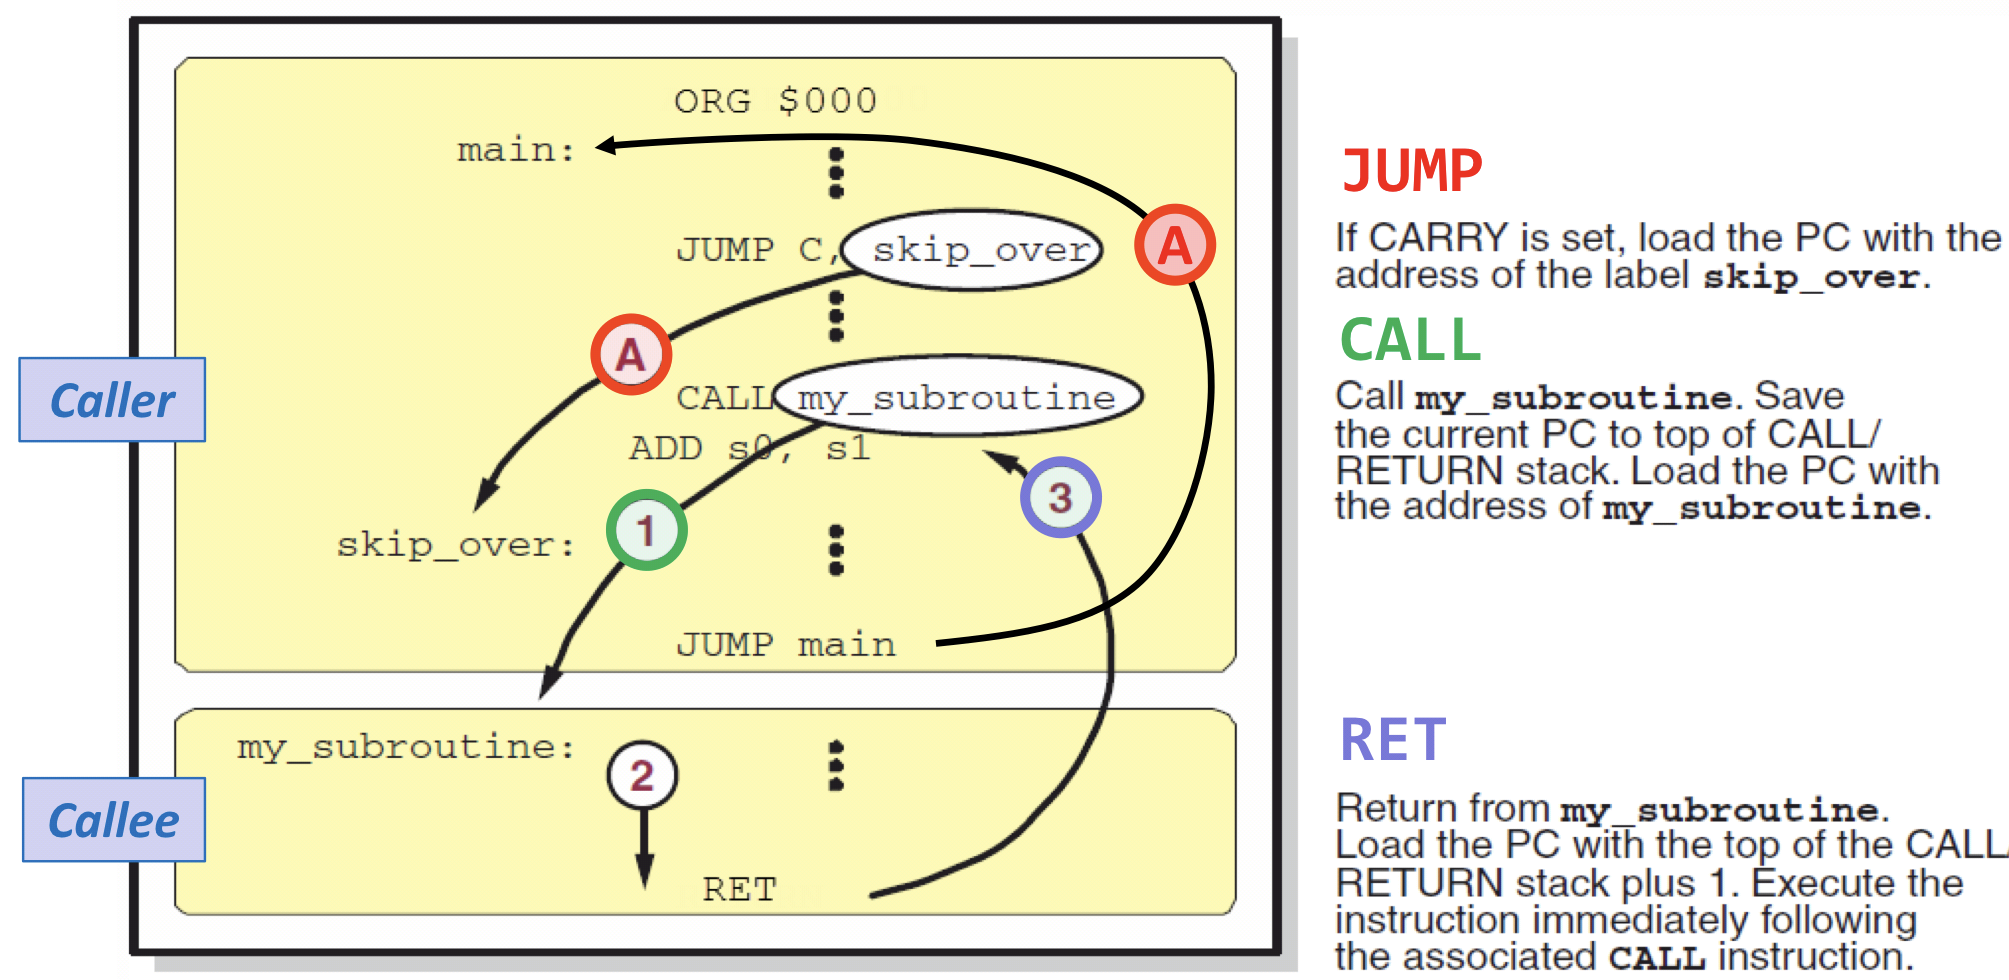
\includegraphics[width=9cm]{pics/Ablauf_Synchron}
\end{minipage}

\subsubsection{Interrupt Instruktionen}
\begin{minipage}{9cm}
	Neben Programm Counter "Anderungen, welche synchron auftreten gibt es auch welche die asynchron auftreten. Dabei wird zwischen Interrupt Event und Reset Event unterschieden.
	
	\textbf{Interrupt Event}
	\begin{itemize}
		\item \textbf{Kann} zu einer Unterbrechung f"uhren
		\item f"uhrt Sprung zum Interrupt-Vektor aus (PC = \$3FF)
		\item R"ucksprungadresse wird auf den CALL/RETURN Stack gelegt
		\item Zust"ande der Flags \textbf{Zero} und \textbf{Carry} werden gesichert, das Interrupt Enable Flag wird gel"oscht (\textbf{IE=0})
	\end{itemize}
	\textbf{Reset Event}
	\begin{itemize}
		\item f"uhrt \textbf{immer} zu einem Neustart des PicoBlaze
		\item PC wird r"uckgesetzt (PC = \$000)
		\item l"oscht die Flags Zero, Carry und IE und den CALL/RETURN Stack
		\item General Purpose Regsiter und ScratchPad RAM werden nicht modifiziert
	\end{itemize}
\end{minipage}
%
\begin{minipage}{0.5cm}
	\ \
\end{minipage}
%
\begin{minipage}{9cm}
	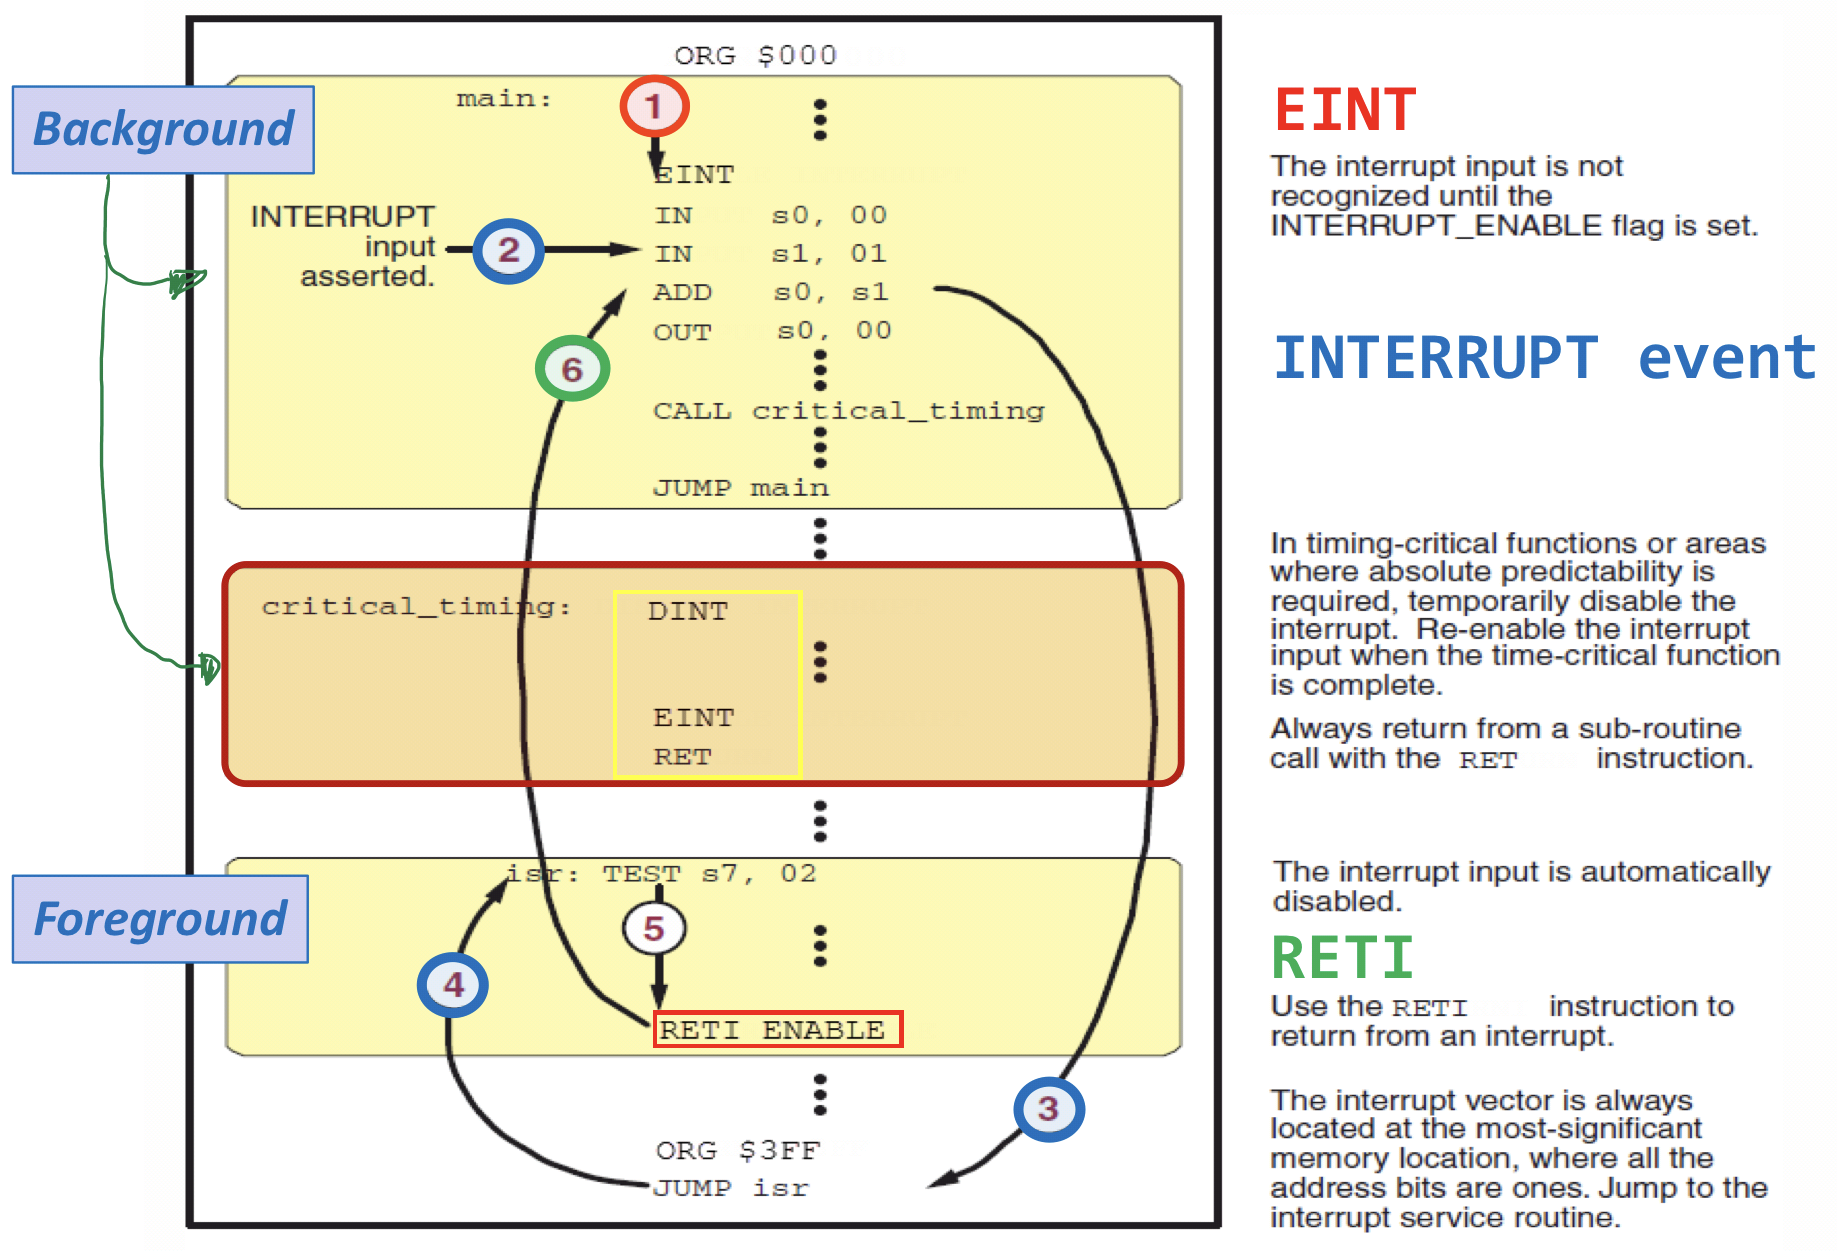
\includegraphics[width=9cm]{pics/Ablauf_Asynchron}
\end{minipage}
\newpage